\documentclass{article}
\usepackage{amsmath,tikz,algorithm2e,amssymb}
\usetikzlibrary{matrix,calc}
\title{Computer\/ Robot Vision: Lecture 5}
\author{Sam Barrett}

\begin{document}
\maketitle

\section{Feature-Based alignment}

Feature based alignment can be used to match known objects in a cluttered scene. It can also be used in enhancing medical imaging by combining multiple images into more detailed, accurate images.

We have previously seen how to fit a model to image evidence in the form of matching a line to edge points. Here, we will fit the parameters of some transformation according to a set of matching feature pairs, i.e. we will be able to work out what transformation an image has undergone to produce another image with matching features.

\subsection{Parametric (global) warping}

Parametric warping is a form of warping and can be caused by:

\begin{itemize}
  \item translation
  \item rotation
  \item aspect shift
  \item affine shift
  \item perspective shift
\end{itemize}

These are all examples of transformations and so can be thought as a black-box operator which takes an image and returns a altered image.

Mathematically, this can be thought of as:

\[
 \mathbf{p'}_{x',y'}= T(\mathbf{p}_{x,y})
\]

For some transformation or \textit{coordinate-changing machine} $T$.

$T$ being \textbf{global} tells us:

\begin{itemize}
  \item It is the same for any point $p$
  \item It can be described parametrically
\end{itemize}

We can represent $T$ as a matrix $\mathbf{M}$, and we can then rewrite our transformation of $p$ to $p'$ as:

\[
  p' = \mathbf{M} p
\]

or

\[
  \begin{bmatrix}
    x' \\ y'
  \end{bmatrix} =
  \mathbf{M} \begin{bmatrix}
    x \\ y
  \end{bmatrix}
\]

\paragraph{Scaling} a coordinate means multiplying each of its components by a scalar.

\paragraph{Uniform scaling} means this scalar is the same for all components

\paragraph{Non-uniform scaling} means that different scalars apply to different components (where components are dimensions).

Scaling can be represented as:

\begin{align*}
  x' &= ax \\
  y' &= by
\end{align*}

or in matrix form:

\[
  \begin{bmatrix}
    x'\\ y'
  \end{bmatrix} =
  \underbrace{\begin{bmatrix}
    a & 0 \\
    0 & b
  \end{bmatrix}}_{\text{Scaling matrix $S$}}\begin{bmatrix}
    x \\ y
  \end{bmatrix}
\]

Using a 2x2 matrix as seen above, we can represent:

\begin{itemize}
  \item 2D scaling

        \begin{align*}
          x' = s_{x}x \\
          y' = s_{y}y
        \end{align*}
\[
  \begin{bmatrix}
    x'\\ y'
  \end{bmatrix} =
  \begin{bmatrix}
    s_{x} & 0 \\
    0 & s_{y}
  \end{bmatrix}\begin{bmatrix}
    x \\ y
  \end{bmatrix}
        \]
  \item 2D rotation around $(0,0)$

        \begin{align*}
          x' = \cos(\Theta)x - \sin(\Theta)y \\
          y' = \sin(\Theta)x + \cos(\Theta)y
        \end{align*}
\[
  \begin{bmatrix}
    x'\\ y'
  \end{bmatrix} =
  \begin{bmatrix}
    \cos\Theta & -\sin\Theta \\
    \sin\Theta & \cos\Theta
  \end{bmatrix}\begin{bmatrix}
    x \\ y
  \end{bmatrix}
        \]
  \item 2D shear

        \begin{align*}
          x' = x + sh_{x} \times y\\
          y' = sh_{y} \times x + y
        \end{align*}
\[
  \begin{bmatrix}
    x'\\ y'
  \end{bmatrix} =
  \begin{bmatrix}
    1 & sh_{x} \\
    sh_{y} & 1
  \end{bmatrix}\begin{bmatrix}
    x \\ y
  \end{bmatrix}
        \]

  \item 2D mirror about Y axis

        \begin{align*}
          x' = -x\\
          y' = y
        \end{align*}
\[
  \begin{bmatrix}
    x'\\ y'
  \end{bmatrix} =
  \begin{bmatrix}
    -1 & 0 \\
    0 & 1
  \end{bmatrix}\begin{bmatrix}
    x \\ y
  \end{bmatrix}
        \]

  \item 2D Mirror about $(0,0)$

        \begin{align*}
          x' = -x\\
          y' = -y
        \end{align*}
\[
  \begin{bmatrix}
    x'\\ y'
  \end{bmatrix} =
  \begin{bmatrix}
    -1 & 0 \\
    0 & -1
  \end{bmatrix}\begin{bmatrix}
    x \\ y
  \end{bmatrix}
        \]
  \item 2D translation

       \begin{align*}
         x' = x + t_{x}\\
         y' = y + t_{y}
       \end{align*}

        \textbf{NOTE: 2D translation cannot be represented in matrix form}
\end{itemize}

From this we can see that 2D linear transformations can be represented using a $2\times 2$ matrix.

Linear transformations are combinations of:

\begin{itemize}
  \item scale
  \item rotation
  \item shear
  \item mirror
\end{itemize}

\subsection{Homogeneous coordinates}

These are a convenient coordinate system to use to represent transformations.

To convert to this system we add an extra dimension to our points, defaulted at 1.

\[
  (x,y) \to \begin{bmatrix}
    x \\ y \\ 1
  \end{bmatrix}
\]

To convert \textbf{from} homogeneous coordinates:

\[
  \begin{bmatrix}
    x \\ y \\ w
  \end{bmatrix} \to \left(\frac{x}{w}, \frac{y}{w} \right)
\]


Using this system we can represent 2D translations in matrix form, using $3\times 3$ matrices.

\begin{align*}
  x' = x + t_{x} \\
  y' = y + t_{y}
\end{align*}

This translation matrix can now be represented as:

\[
  \begin{bmatrix}
    1 & 0 & t_{x} \\
    0 & 1 & t_{y} \\
    0 & 0 & 1
  \end{bmatrix}
\]

Leading to translations of the form:

\[
  \begin{bmatrix}
    x' \\ y' \\ 1
  \end{bmatrix} =
  \begin{bmatrix}
    1 & 0 & t_{x} \\
    0 & 1 & t_{y} \\
    0 & 0 & 1
  \end{bmatrix}
  \begin{bmatrix}
    x \\ y \\ 1
  \end{bmatrix} =
  \begin{bmatrix}
    x + t_x \\
    y + t_y \\
    1
  \end{bmatrix}
\]

We can re-format our basic 2D transformations seen earlier into transformations in the homogeneous coordinate space:

\begin{itemize}
  \item Scale

        \[
        \begin{bmatrix}
    x' \\ y' \\ 1
  \end{bmatrix} =
  \begin{bmatrix}
    s_{x} & 0 & 0 \\
    0 & s_{y} & 0 \\
    0 & 0 & 1
  \end{bmatrix}
  \begin{bmatrix}
    x \\ y \\ 1
  \end{bmatrix}
        \]
  \item Rotation

        \[
        \begin{bmatrix}
    x' \\ y' \\ 1
  \end{bmatrix} =
        \begin{bmatrix}
          \cos\Theta & -\sin\Theta & 0 \\
          \sin\Theta & \cos\Theta & 0 \\
          0 & 0 & 1
  \end{bmatrix}
  \begin{bmatrix}
    x \\ y \\ 1
  \end{bmatrix}
        \]
  \item Shear

        \[
        \begin{bmatrix}
    x' \\ y' \\ 1
  \end{bmatrix} =
        \begin{bmatrix}
          1 & sh_{x} & 0 \\
          sh_{y} & 1 & 0 \\
          0 & 0 & 1
  \end{bmatrix}
  \begin{bmatrix}
    x \\ y \\ 1
  \end{bmatrix}
        \]

\end{itemize}

\subsection{2D Affine Transformations}

An affine transformation is a combination of both Linear transformations and translations and have the general form of:

\[
  \begin{bmatrix}
    x' \\ y' \\ w'
  \end{bmatrix} =
  \begin{bmatrix}
    a & b & c \\
    d & e & f \\
    0 & 0 & 1
  \end{bmatrix}\begin{bmatrix}
    x \\ y \\ w
  \end{bmatrix}
\]

When using these transformations, \textbf{parallel lines are preserved.}


\section{Affine Fit}

Image alignment approaches fall into two broad categories:

\begin{enumerate}
  \item Direct (pixel-based) alignment

        Here we search for the alignment where most pixels \textit{agree}


  \item Feature-based alignment

        Here we search for alignment based on where extracted features \textit{agree}. Our result can then be verified by direct alignment.
\end{enumerate}

\subsection{Fitting an Affine transformation}

Assume that we know the pixel correspondences between two images. How do we work out the transformation $T$ which maps the first image to the second?

In

\[
  \begin{bmatrix}
    x_{i }' \\ y_{i}'
  \end{bmatrix}
  = \begin{bmatrix}
    m_{1} & m_{2} \\
    m_{3} & m_{4}
  \end{bmatrix}\begin{bmatrix}
    x_{i}\\
    y_{i}
  \end{bmatrix} + \begin{bmatrix}
    t_{1} \\ t_{2}
  \end{bmatrix}
\]

We want to find $m_{1..4}$ and $t_{1..2}$

We can start by rewriting our equation to the form:

\[
  \begin{bmatrix}
    & & \ldots & & & \\
    x_{i} & y_{i} & 0 & 0 & 1 & 0 \\
    0 & 0 & x_{i} & y_{i} & 0 & 1 \\
     & & \ldots & & &
   \end{bmatrix}
   \begin{bmatrix}
     m_{1} \\ m_{2} \\ m_{3} \\ m_{4} \\ t_{1} \\ t_{2}
   \end{bmatrix}=
   \begin{bmatrix}
     \ldots \\ x_{i}' \\ x_{i}' \\ \ldots
   \end{bmatrix}
 \]

 How many pixel correspondences do we need to solve this for the transformation parameters (the values of the 1x6 matrix)? We require 3 corresponding pairs.

 Once we have these values, we can easily calculate the corresponding point of a point in either image. Say we want to find the corresponding point of $(x_{new},y_{new})$ we would calculate the following:

\[
  \begin{bmatrix}
    & & \ldots & & & \\
    x_{new} & y_{new} & 0 & 0 & 1 & 0 \\
    0 & 0 & x_{new} & y_{new} & 0 & 1 \\
     & & \ldots & & &
   \end{bmatrix}
   \begin{bmatrix}
     m_{1} \\ m_{2} \\ m_{3} \\ m_{4} \\ t_{1} \\ t_{2}
   \end{bmatrix}=
   \begin{bmatrix}
     \ldots \\ x_{new}' \\ x_{new}' \\ \ldots
   \end{bmatrix}
 \]

 But where do we get the initial 3 corresponding pairs?

 One method is to scan the entire second image for a match for a single point in the first. Similarity between two patches can be calculated as the \textit{Sum of Squared Differences (SSD)}. However, this is clearly very computationally expensive. Another alternative is called \textbf{SIFT}, we will not go into detail.

 \section{RANSAC}

 We require a more robust method for dealing with outliers. Large disagreements in a small subset of points can cause failure in least-squares based approaches. This can happen often as a lot of data in computer vision suffers from noise, in some cases over half of the data is expected to be outliers!

 Outliers can result in the erroneous pairing of points in two images.

 RANSAC stands for: \textbf{RAN}dom \textbf{S}ample \textbf{C}onsensus. It is very popular as it is generalisable and simple to implement. It is robust against large proportions of outliers.

 The general approach of RANSAC is to ignore outliers. Intuitively we say that if an outlier is chosen to compute the current fit, then the resulting line won't have much \textit{support} from the rest of the points.

 The algorithm has the general form:

 \begin{algorithm}
   \While{iterations $<$ maxIterations}{
     Randomly select minimal subset of points as a \textit{seed} group

     Compute a model using these points

     \For{each point}{
       calculate error wrt. this model

       Select all points \textit{consistent} with this model, i.e. points that fit with the model within some tolerance.
     }
 }
 \Return model with largest number of inliers, largest number of supporting points
 \end{algorithm}

 We can apply this to our transformation fitting example.

 \begin{enumerate}
   \item Randomly select the smallest group of point correspondences from which we can estimate the parameters of our model

   \item Fit the parametric mode to the selected correspondences

   \item Count how many of all correspondences are in agreement, this is the number of inliers

 \end{enumerate}

 We repeat the above for a set number of iterations and return the model with the highest number of correspondences supporting it.

 \section{Panoramic Images}

 The basic process for creating a panorama (or mosaic) is as follows:

 \begin{itemize}
\item Take a sequence of images from the same position
   \item compute transformation between second and first image
   \item transform the second image to overlap with the first
   \item blend the two images
   \item repeat for all images
 \end{itemize}


 Abstractly, when creating a panoramic image, we are moving the plane on which the real camera location exist to a synthetic plane on which the images line up. This can be done as long as all images have the same centre of projection. (See Figure~\ref{fig:synthview})

\begin{figure}[ht]
  \centering
  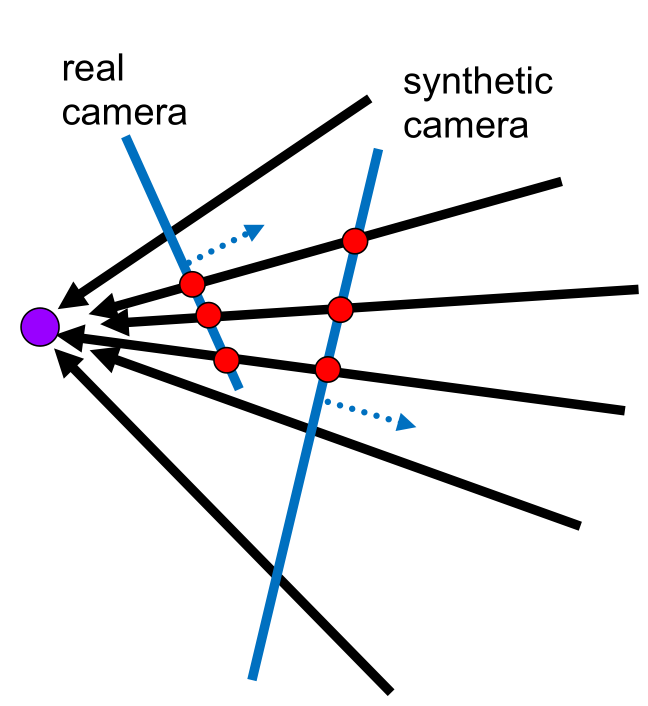
\includegraphics[scale=0.4]{figures/l5-1.png}
  \caption{\label{fig:synthview} Generating synthetic views}
\end{figure}

We can think of our mosaic as a synthetic wide-angle camera. We re-project our images onto a common plane on which the mosaic is formed.

In order to map a pixel from one image to another from the same image centre, we can cast a ray through each pixel in the first image and overlay it where it passes through the second image. This can be seen more clearly in Figure~\ref{fig:raytrace}

\begin{figure}[ht]
  \centering
  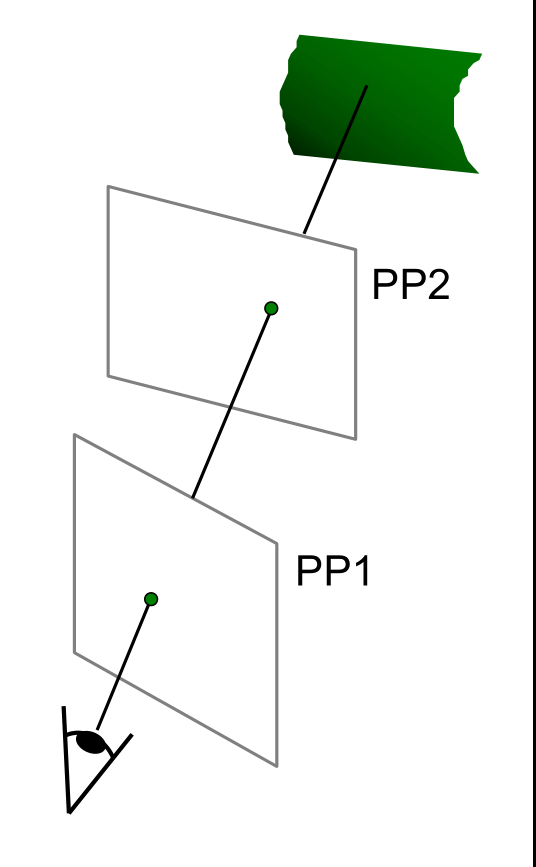
\includegraphics[scale=0.4]{figures/l5-2.png}
  \caption{\label{fig:raytrace} }
\end{figure}



We can consider our re-projection as a 2D image warp from one image to another instead of as a 3D re-projection.


\subsection{Image re--projection: Homography}

A projective transform is a \textbf{mapping between any two perspective projections with the same centre of projection}

Any rectangle should map to an arbitrary quadrilateral, parallel lines are not preserved but straight lines are. This process is called \textbf{homography} and has the general mathematical form:

\[
  \underbrace{\begin{bmatrix}
    wx' \\ wy' \\ w
  \end{bmatrix}}_{\mathbf{p'} } =
\underbrace{\begin{bmatrix}
  *&*&*\\ *&*&* \\ *&*&*
\end{bmatrix}}_{\mathbf{H} }\underbrace{\begin{bmatrix}
x \\ y \\ 1
\end{bmatrix}}_{\mathbf{p} }
\]

\subsection{The projective plane}

We again employ homogeneous coordinates. These allow us to represent points at infinity, homographies, perspective projection and multi-view relationships.

Geometrically, we can say that a point in the image corresponds to a ray in the projective space. (See Figure~\ref{fig:projectiveplane})

We can say that each point in the image $(x,y)$ is represented by a ray $(sx,sy,s)$ in the projective plane. \textbf{All points on the ray are equivalent $(x,y,1) \equiv (sx,sy,s)$}

\begin{figure}[ht]
  \centering
  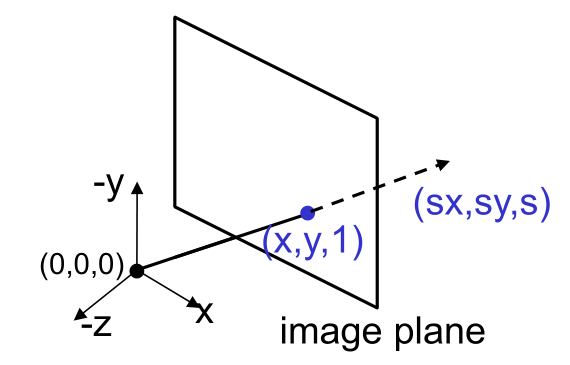
\includegraphics[scale=0.4]{figures/l5-3.png}
  \caption{\label{fig:projectiveplane} Image point in the projective plane}
\end{figure}

\subsection{Solving for Homographies}

We now want to attempt to solve the equation outlined earlier:

\[
  \mathbf{p' = Hp}
\]

\[
  \begin{bmatrix}
    wx' \\ wy' \\ w
  \end{bmatrix} =
  \begin{bmatrix}
    h_{00} & h_{01} & h_{02} \\
    h_{10} & h_{11} & h_{12} \\
    h_{20} & h_{21} & h_{22} \\
  \end{bmatrix}\begin{bmatrix}
    x \\ y \\ 1
  \end{bmatrix}
\]


up to some scale factor determined by the \textbf{Frobenius norm} of $\mathbf{H}$ being 1.

  We define the Frobenius norm as follows:

  \[
    \| A \|_{F} \equiv \sqrt{\sum_{i=1}^m \sum_{j=1}^n |a_{ij}|^{2} } = \sqrt{\text{Tr}(\mathbf{A}\mathbf{A}^{H}  )}
  \]

  Where $\mathbf{A}^{H} $ is known as the conjugate transpose and $\text{Tr}(\mathbf{A} ) = \sum_{i=1}^n a_{ii}$

  The conjugate transpose is a matrix $\mathbf{A} $ is found by taking the transpose of $\mathbf{A} $ and then taking the complex conjugate of each element in $\mathbf{A}^{T} $. The complex conjugate being, for $a + ib$, $a - ib$


  We therefore, formulate the problem:

  \[
    \min\|Ah-b\|^{2}
  \]

  s.t. $\|h\|^{2}=1$

  Where $h$ is a vector of unknowns $h =  \begin{bmatrix}
    h_{00} & h_{01} & h_{02} &
    h_{10} & h_{11} & h_{12} &
    h_{20} & h_{21} & h_{22}
  \end{bmatrix}^{T}$

  \section{2D Image warping}

  Given a source image $f$ and a transform $T$, how do we compute the transformed image $g = T(f)$? We can send each pixel $f(x,y)$ to the corresponding location $(x',y')=T(x,y) $ in the second image. But sometimes $T(x,y)$ produces a location \textit{between} pixel values.

  In this case we distribute the colour of $f(x,y)$ between the neighbouring pixels, this is known as \textbf{splatting}.

  \subsection{Inverse warping}

When performing the reverse procedure, if a pixel value comes from between two pixels, we interpolate its colour from surrounding pixels. There are different types of interpolation: nearest neighbour, bilinear, etc.

\section{Changing camera centre}

We have stated previously that our transformations work when we have a common camera centre for all the images we are attempting to stitch together.

However, we can still perform these operations if our camera centre were to change but only if the (3rd) projection plane is sufficiently far away from all camera centres. This is how large-scale aerial photographs are taken.

\section{RANSAC for estimating homography}

We can use RANSAC for estimating $H$ as defined in our earlier equations. The general approach for this is as follows:

\begin{enumerate}
  \item Select feature pairs at random
  \item Compute exact homography, $H$
  \item Compute inliers, pairs where $SSD(p_{i}', \mathbf{H}p_{i} ) < \varepsilon$
  \item Keep largest set of inliers
  \item Re-compute least-squares $H$ estimate on all inliers
\end{enumerate}

\section{Local Features}

The main components of local features are as follows:

\begin{enumerate}
\item Detection, being able to identify the points of interest in an image
  \item Description, being able to extract a feature vector (descriptor) describing the surrounding of each point of interest.
  \item Matching, being able to determine the correspondence between two descriptors in two views.
\end{enumerate}

With these components we desire the following properties:

\begin{itemize}
  \item Repeatability: We want the same features to be found in several images despite geometric and photometric transformations.

        This would likely not happen if we were to simply employ random sampling. We require this to be the case at least partially as we must run detection separately on each image.

  \item Saliency: Each feature should have a distinctive description

        We want to be able to reliably determine which point goes with which. To achieve this, we must provide some invariance to geometric and photometric differences between the two views

  \item Compactness and efficiency: We want to find far fewer features than there are image pixels
  \item Locality: A feature occupies a relatively small area of the image and is robust against clutter and occlusion.
\end{itemize}

Image features have found uses in image alignment, 3D image reconstruction, motion tracking and robot navigation to name a few.

\subsection{Key Point Detection}

There are a number of keypoint detectors, including \textit{Hessian \& Harris}, \textit{Laplacian, DoG} and many others.

Corners are widely considered to make good keypoints, they are repetitive and distinctive and can be easily recognised using a relatively small kernel. Windows around a corner should see large changes in gradient and gradient direction.

\subsubsection{Harris corner detector}

This detector is based on the intensity change for a shift $[u,v]$

\[
  E(u,v) = \sum_{x,y} w(x,y) [I(x+u,y+v) - I(x,y)]^{2}
\]

Where:

\begin{itemize}
  \item $w$ is the weight function and $w(x,y)$ is the weight at a point $(x,y)$

        The weight function can be anything but a common one is a Gaussian kernel

  \item $I(x+u,y+v)$ is the intensity after the shift
  \item $I(x,y)$ is the intensity before the shift.
\end{itemize}

For small shifts, $E$ can be linearly approximated as:

\[
  E(u,v) \approx \begin{bmatrix}
    u & v
  \end{bmatrix}
 M \begin{bmatrix}
    u\\ v
  \end{bmatrix}
\]

With $M$ being a $2 \times 2$ matrix of image derivatives:

\[
  M = \sum_{x,y} w(x,y) \begin{bmatrix}
    I_{x}(x,y)I_{x}(x,y) & I_{x}(x,y)I_{y}(x,y) \\
    I_{x}(x,y)I_{y}(x,y) & I_{y}(x,y)I_{y}(x,y)
  \end{bmatrix}
\]

This can be further optimised by replacing the summation with a convolution by a Gaussian kernel:

\[
  M = \begin{bmatrix}
    G(\sigma)\star I_{x}^{2} & G(\sigma)\star I_{x}I)_{y} \\
    G(\sigma)\star I_{x}I_{y} & G(\sigma)\star I_{y}^{2}
  \end{bmatrix} =
  G(\sigma) \star \begin{bmatrix}
    I_{x}^{2} & I_{x}I_{y} \\
    I_{x}I_{y} & I_{y}^{2}
  \end{bmatrix}
\]

\subsubsection{Eigenvectors \& Eigenvalues}

The general form of eigenvalues and eigenvectors is:

\[
  M \mathbf{e} = \lambda \mathbf{e}
\]

Where $\mathbf{e}$ is an eigenvector and $\lambda$ is an eigenvalue.

Most vectors change direction when multiplied by a matrix $M$, however, certain exceptions exist. These are known as eigenvectors. In these cases multiplying our vector $\mathbf{e} $ by $M$ is the same as multiplying $\mathbf{e} $ by a scalar $\lambda$, this is known as a eigenvalue. This tells us whether (and how) $\mathbf{e} $ is changed when multiplied by $M$, it can be any change other than a change in direction.


We can rewrite this as:

\[
  (M - \lambda I)\mathbf{e} = 0
\]

Where $I$ is the identity matrix.

To calculate the eigenvector, we must:

\begin{enumerate}
  \item Compute the determinant of $M-\lambda I$, the result of which is a polynomial
  \item Find the roots of the polynomial, i.e. solve $\text{det}(M-\lambda I) =0$, this returns our eigenvalues
  \item For each eigenvalue, solve $(M-\lambda I)\mathbf{e} = 0 $ for $\mathbf{e} $
\end{enumerate}



\subsubsection{Covariance matrix analysis}

We can decompose our covariance matrix $M$ into eigenvectors and eigenvalues:

\[
  M = R \begin{bmatrix}
    \lambda_{max} & 0 \\
    0 & \lambda_{min}
  \end{bmatrix}R^{T}
\]




\end{document}
